\documentclass[10pt,a4paper]{article}
\usepackage[utf8]{inputenc}
\usepackage{amsmath}
\usepackage{amsfonts}
\usepackage{amssymb}
\usepackage{makeidx}
\usepackage{graphicx}
\usepackage[left=2cm,right=2cm,top=2cm,bottom=2cm]{geometry}
\author{Universidad Politécnica De La Zona Metroplitana de Guadalajara \\\\ Integrantes:\\ Jiménez Cortés Raúl \\ Díaz Fuentes Miguel Ángel Xamie \\\\ Carrera:\\ Ingeniería Mecatrónica\\\\ Grupo:\\ 4ª "B" \\\\
Materia:\\ Sistemas Electrónicos De Interfaz \\\\ Profesor:\\ Morán Garabito Carlos Enrique}
\title{EV-1-1-CIRCUITOS DE REFTIFICACÓN NO CONTROLADOS}
\date{20/Septiembre/2019}


\begin{document}
\begin{figure}
\centering

\includegraphics[scale=1]{Pa.jpg}
\end{figure}

\maketitle

\newpage
\section{Objetivo}
Desarrollo de problemas de circuitos rectificadores y obtener los resultados por medio del programa de Orcad. 
\section{Materiales}
-Laptop\\ -Programa Orcad instalado\\ -PDF de problemas
\section{Procedimiento}
En la practica que se llevo a cabo su realizacion se anexaran por puntos los cuales son del 1.2-1.7.
\subsection{1.2.-Rectificador De Media Onda Con Carga Inductiva}
En este circuito se pondran algunos elementos de la rectificación no controlada en donde incluiremos una fuente de tensión el cual tendra una vampl de 331 v y una frecuencía de 50 Hz, tambien se le agregara un diodo (Dbreak), una resistencia con un valor de 10, una bobina con un valor de 10 mh y la tierra, una vez ya armado el circuito se correra la simulación pero en transient se le acomodaran los datos en el cual correra la simulación con 50u de incio y de terminación con 40 m, así ya una vez acomodado todos los parametros se correra la simulacion y ns presentara la onda efectuada en el cual se puede observar que la tensión de salida se anula hasta que no le hace la corriente de carga, lo que significa que el diodo del semiperiodo rectificador permanece polarizado en directo, incluso durante una porcion del semiperiodo negativo de la tension de entrada y el cual se mostraran en las siguientes figuras del circuito arma y la simulacion de las ondas.

\begin{figure}[hbtp]
\centering
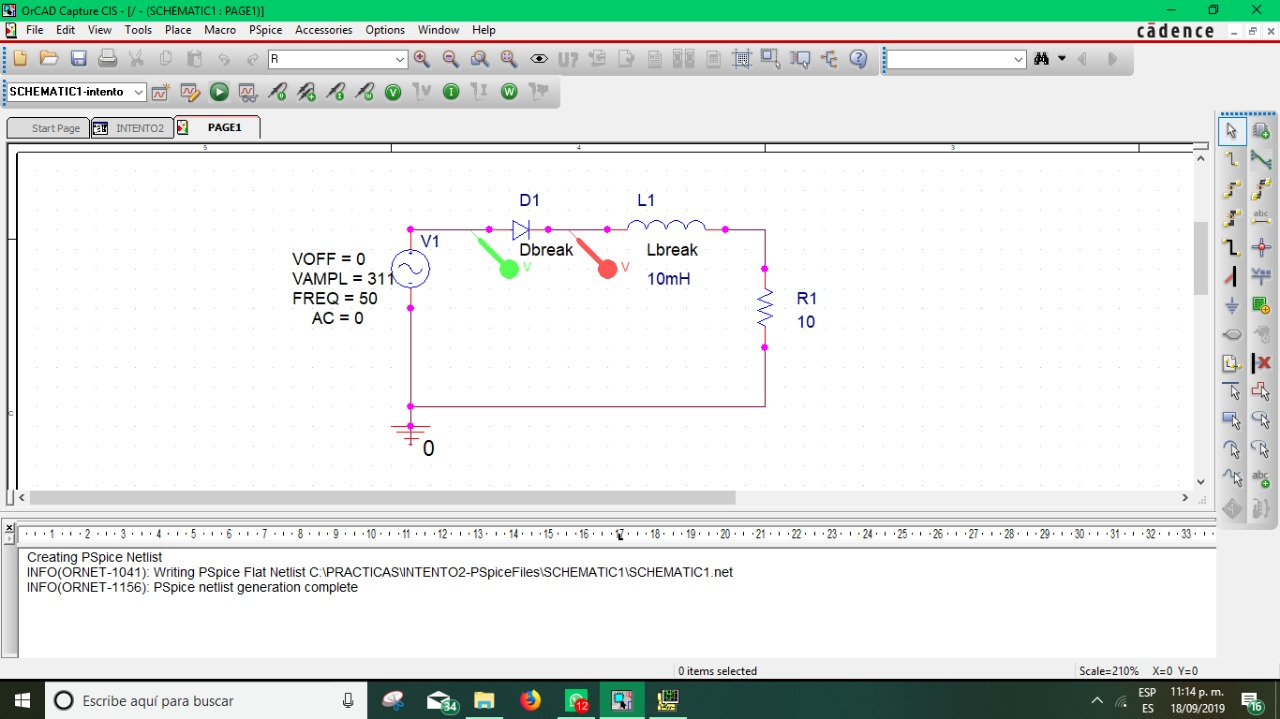
\includegraphics[scale=0.2]{02.jpeg}
\caption{Rectificador De Media Onda Con Carga RL}
\end{figure}
\begin{figure}[hbtp]
\centering
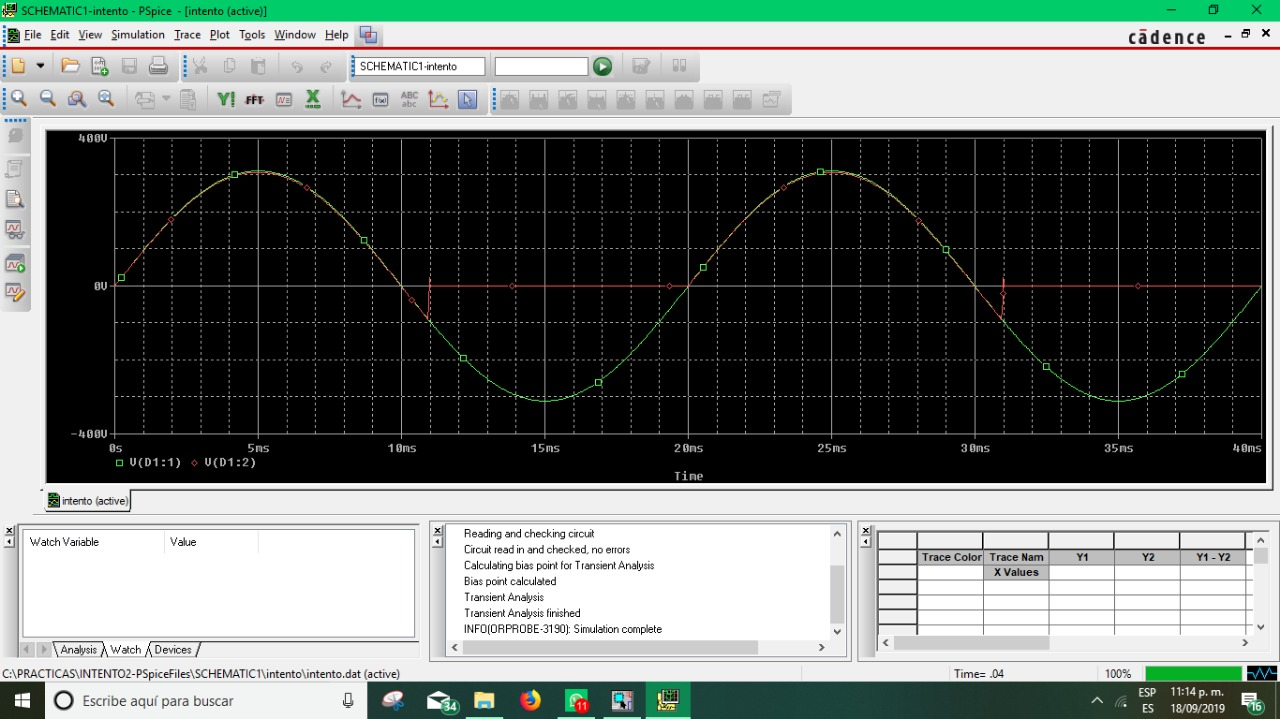
\includegraphics[scale=0.2]{2.jpeg}
\caption{ Simulación: Tensiones De Entrada Y De Salida Del Rectificador}
\end{figure}

\newpage
\subsection{1.3.-Rectificaor Monofásico En Puente}
En este circuito se fomenta un rectificador monofásico el cual es estudiar las principales formas de onda que caracterizan su funcionamiento y determinación electiva de los dispositivos semiconductores (diodos) para asi manifestar  un contenido armonico que el rectificador introduce en la red, en este circuito pondremos una fuente con los valores de vampl de 311v y una frecuencía de 50Hz, tambien se le aregara una bobina, dos resistencias el cual una resistencia tiene un valor de 10m ohm y la otra tiene 10 ohm, cuatro diodos, capacitor con un valor de 1mF y la tierra,una vez ya hecho el circuito de esta manera se efectuara tiempo para que corra la simulacion con un tiempo inicial de 50 us e final con un tiempo de 100ms, llevado a cabo la simulacion se mostrara a continuacion la imagen del circuito junto con la onda generada en la simulación.
\begin{figure}[hbtp]
\centering
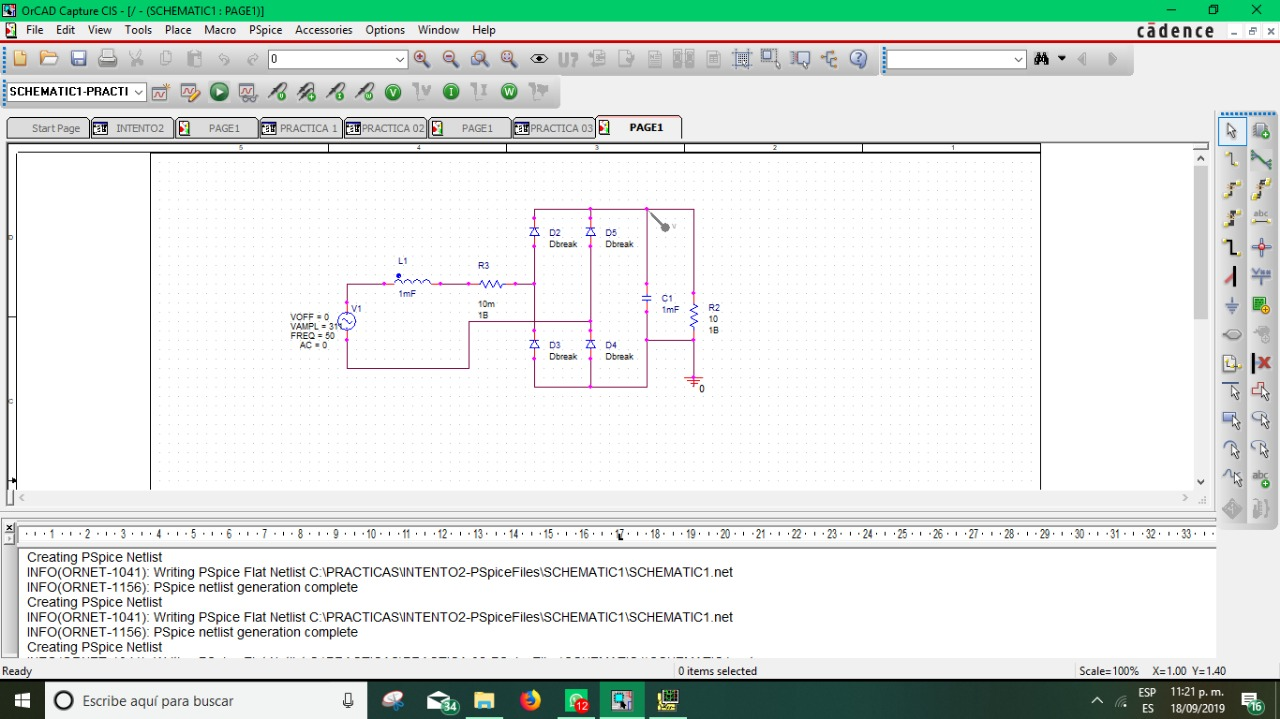
\includegraphics[scale=0.3]{03.jpeg}
\caption{Esquema Del Rectificador Monofásico En Puente}
\end{figure}
\begin{figure}[hbtp]
\centering
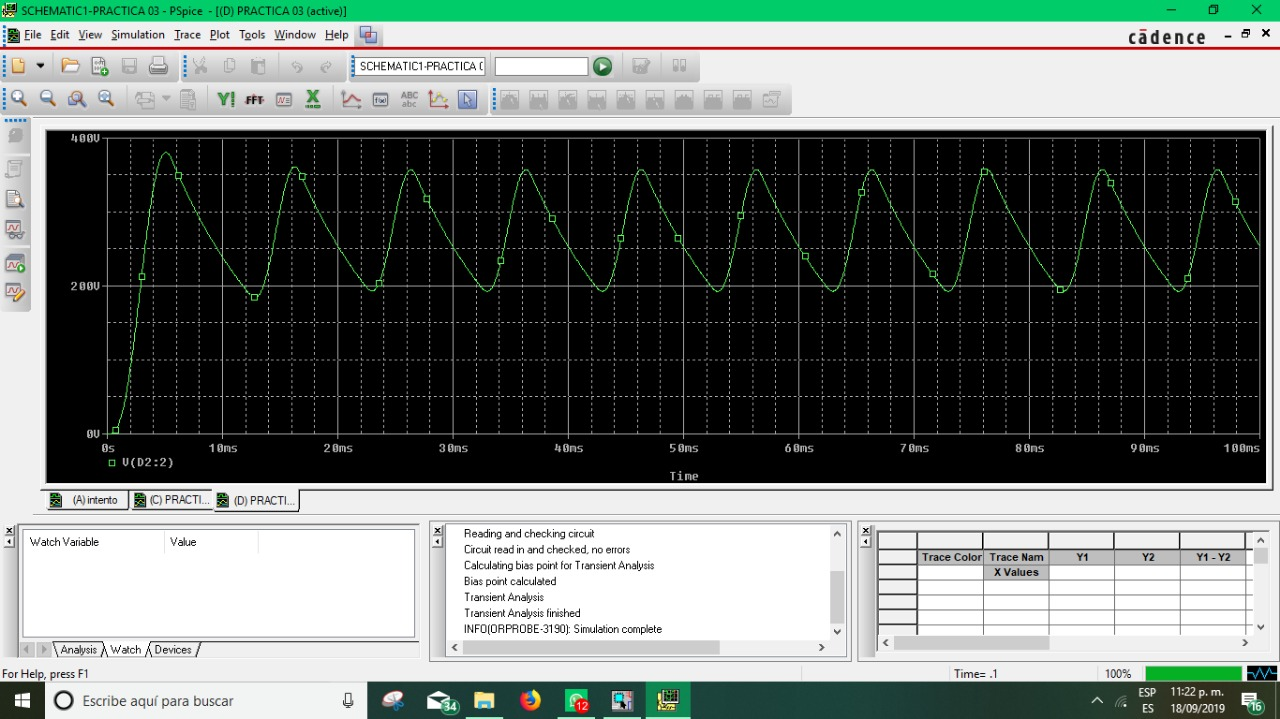
\includegraphics[scale=0.3]{3.jpeg}
\caption{Simulación: Tensión De Salida Del Rectificador}
\end{figure}

\newpage
\subsection{1.4.-Rectificador Monofásico Duplicador De Tensión}
En este punto se obtendran las salidas de una tensión que corresponde el doble de lo que se obtien al punto 1.3 anterior  ya que de esta manera las tensiones son mas elevadas en la etapa continua, en el circuito se le aregara una fuente con un valor de  vamlp:311v y una frecuencia de 50Hz, una bobina con 1mH, dos diodos (Dbreak), dos capacitores con un valor de 1mF, una resistencia con 100 ohm y la tierra, como proseguimiento daremos en correr la simulación el cual se muestran las formas de tensión de salida del rectificador ya que se puede medirse en bornes de los condensadores, como a continuacion se muestra el circuito y la simulación ya que tambien agregamos mas ondas para que se vea un desenfase de cambios de cada onda pero lo importante es la onda de color rojo el cual genera y quiere llegar a obtenerse en este circuito.
\begin{figure}[hbtp]
\centering
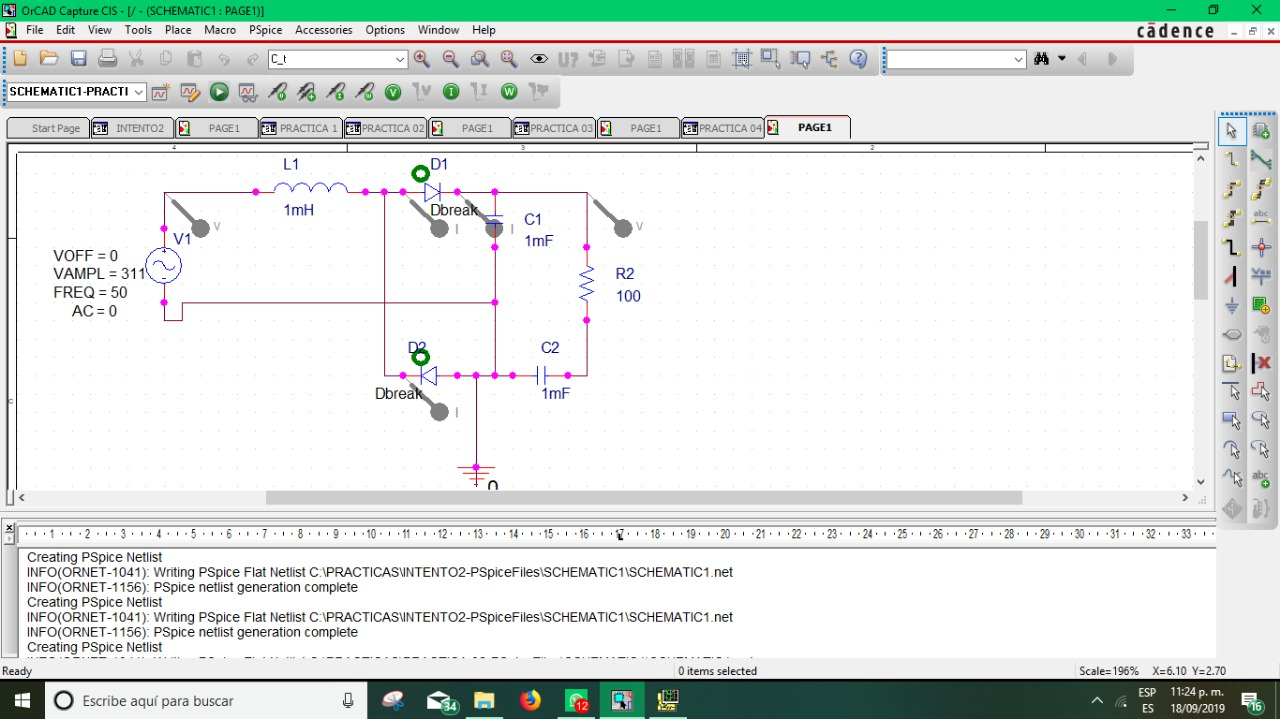
\includegraphics[scale=0.3]{04.jpeg}
\caption{Esquema Del Rectificador Duplicado De Tensión}
\end{figure}
\begin{figure}[hbtp]
\centering
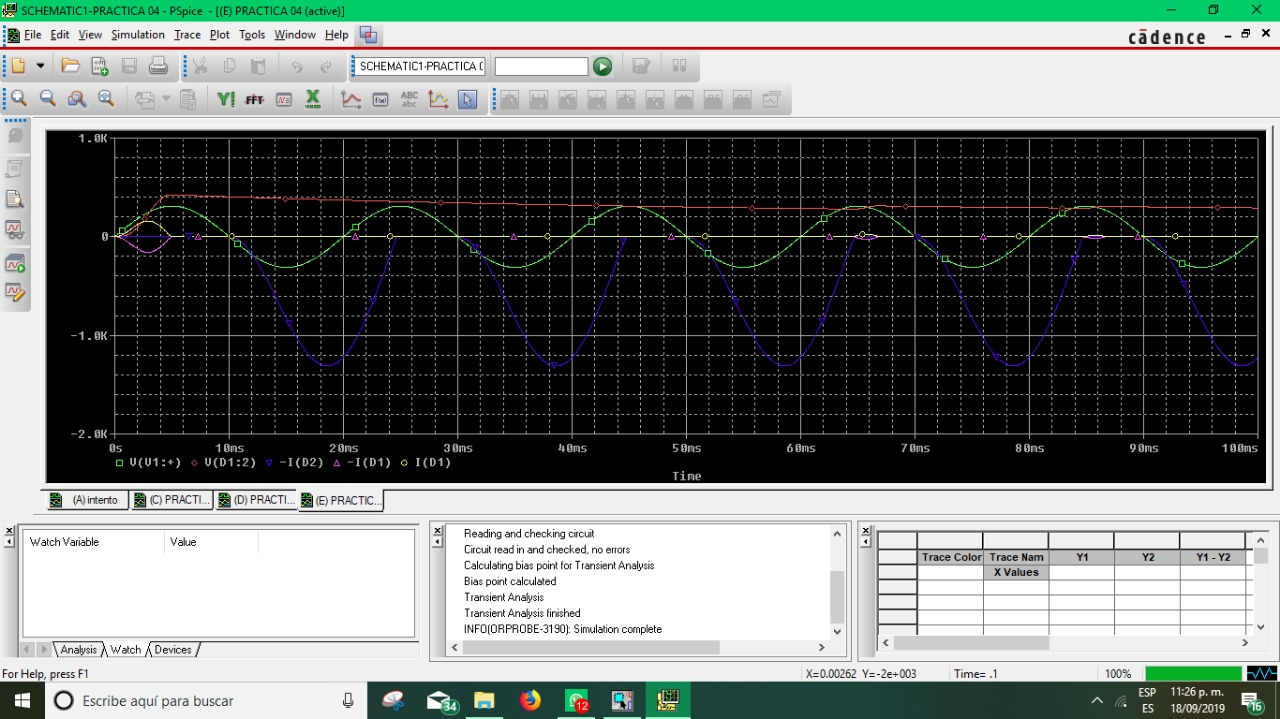
\includegraphics[scale=0.3]{4.jpeg}
\caption{Simulación: Rectificador De Tensión: Tensión De Salida Y En Los Condensadores}
\end{figure}

\newpage
\subsection{1.5.-Efectos De Los Rectificadores Monofásicos En Líneas Trifásicas}
En este punto del presente apartado se fomentaran los incovenientes que se ocasionan los rectificadores monofásicos cuando se conectan a una red trifásica de distribución a 4 hilos (3 fase+neutro), en este punto el reparto de cargas no puede ser exactamente equitativo, siendo que el neutro es el encargado de conducir la corriente de desiquilibrio de los receptores monofásicos,en este circuito se le ah añadido una resistencia de 10 megaohmios e otra de 10 ohm, 4 diodos (Dbreak), un capacitor con un valor de 1mF, una bobina de 1mH,la tierra, una fuente de 220v y 60 Hz, otra de 110v y 60 Hz, y otra de 380v y 60 Hz ya que en este circuito se muestra la fomentacion de las primeras cosas pero en tres partes ya que se mostrara tambien en las simulaciones las diferentes ondas que se fomentan así como se muestran en las siguientes imagenes.
\begin{figure}[hbtp]
\centering
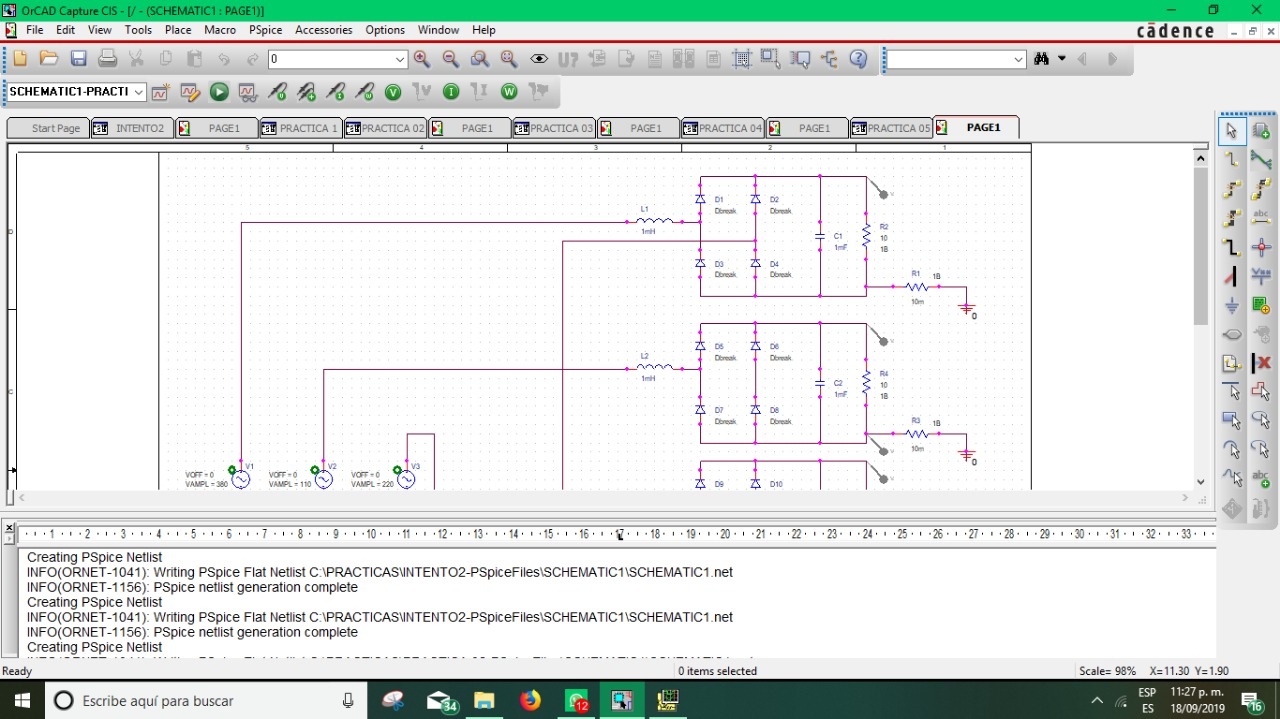
\includegraphics[scale=0.2]{005.jpeg}
\end{figure}
\begin{figure}[hbtp]
\centering
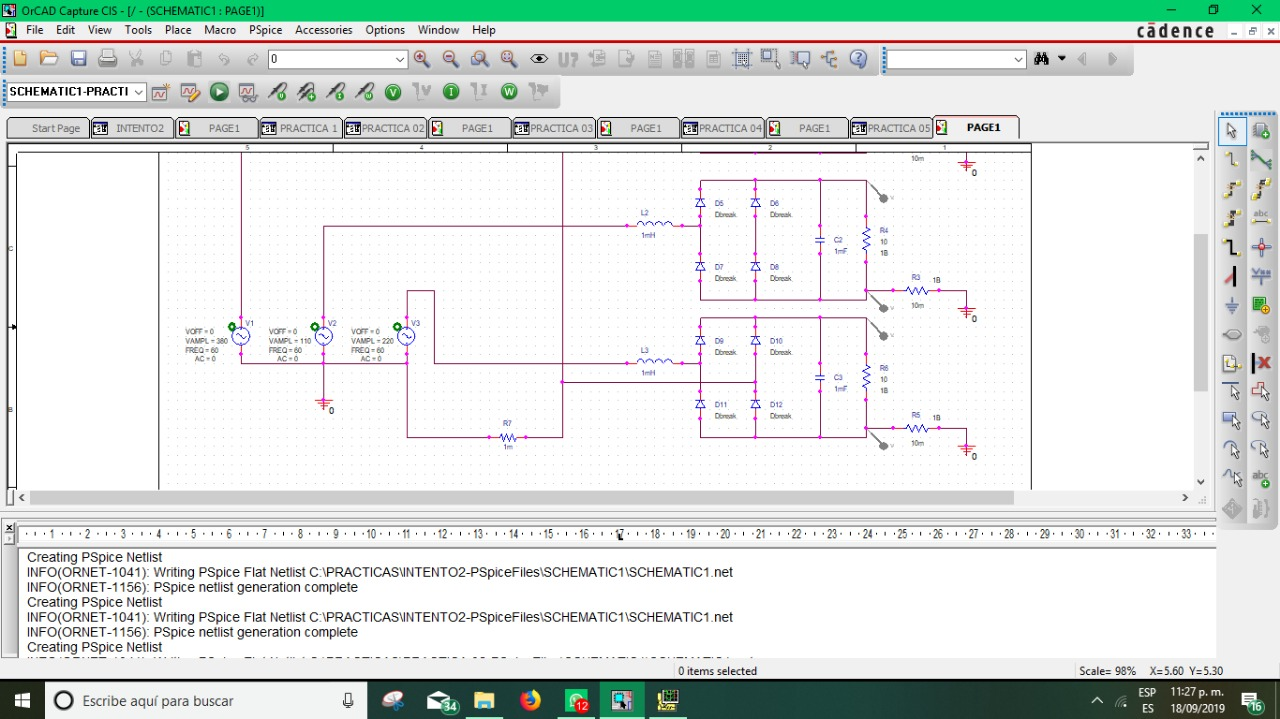
\includegraphics[scale=0.2]{05.jpeg}
\caption{Esquema De Conexión De Tres Monofásicos A Una Línea A 4 Hilos}
\end{figure}
\begin{figure}[hbtp]
\centering
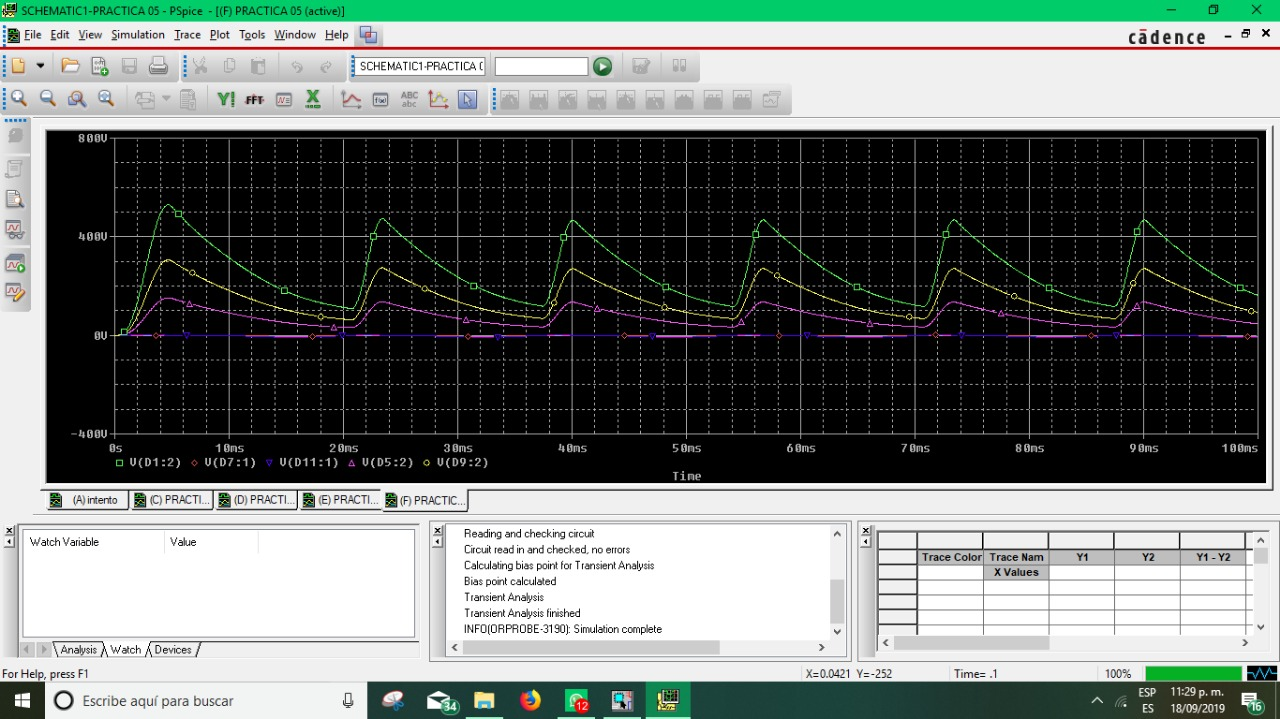
\includegraphics[scale=0.2]{5.jpeg}
\caption{Simulación: Corriente En Los Conductores De Línea Y Su Correspondiente Valor Eficaz}
\end{figure}

\newpage
\subsection{1.6-Rectificadores Trifásicos}
En este punto los rectificadores se utilizan en la forma trifásica ya que cuando la potencia que consume la red es elevada y en estos casos la utilización de rectificadores monofásicos provocan desequilibrios importantes en el consumo de las fases,así que en este punto se mostrara un esquema de un rectificador trifásico no controlado que funciona alimentado por una red de frecuencia de 50Hz y 380v eficaces entre fases y la tensión de salida del rectificador es filtrada mediante por las bobinas y los capacitores, entonces en este circuito se añadiran tres fuentes el cual las tres tiene un valor de 380v y 50Hz pero ya que en ellas se tiene que editar en shistematic la frecuencia enumeradamente del 1-3,las tres bobinas son de 1mH tres resistencias de 1m ohm, 6 diodos (Dbreak), 1 resistencia de 20m ohm y una de 20 ohm tambien se añadira un capacitor de 1mF y una tierra ya que con eso se formara el circuito para un rectificador trifásico no controlado, en la continuación para la simulación se le pondra un tiempo de 50u inicial y 40 m de tiempo final, para asi obtener las diferentes ontas que se muestran a continuación en las imagenes de simulación y el circuito.
\begin{figure}[hbtp]
\centering
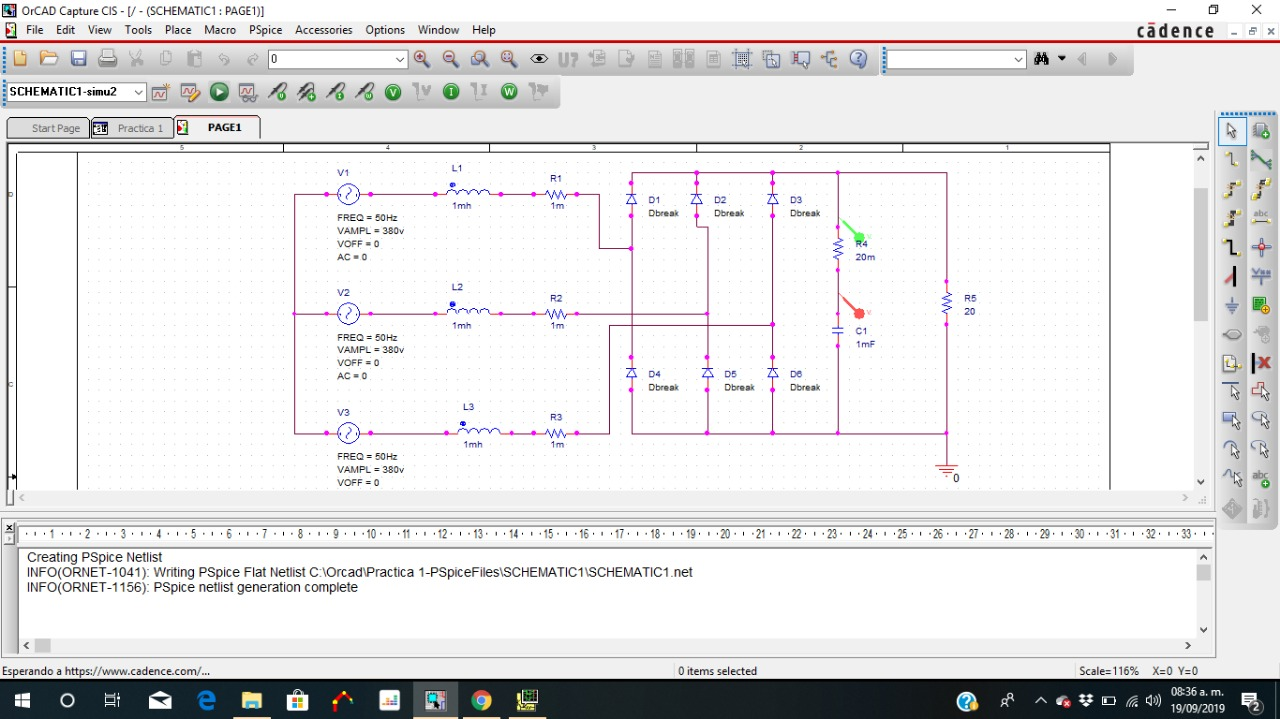
\includegraphics[scale=0.3]{06.jpeg}
\caption{Esquema De Rectificador Trifásico No Controlado}
\end{figure}
\begin{figure}[hbtp]
\centering
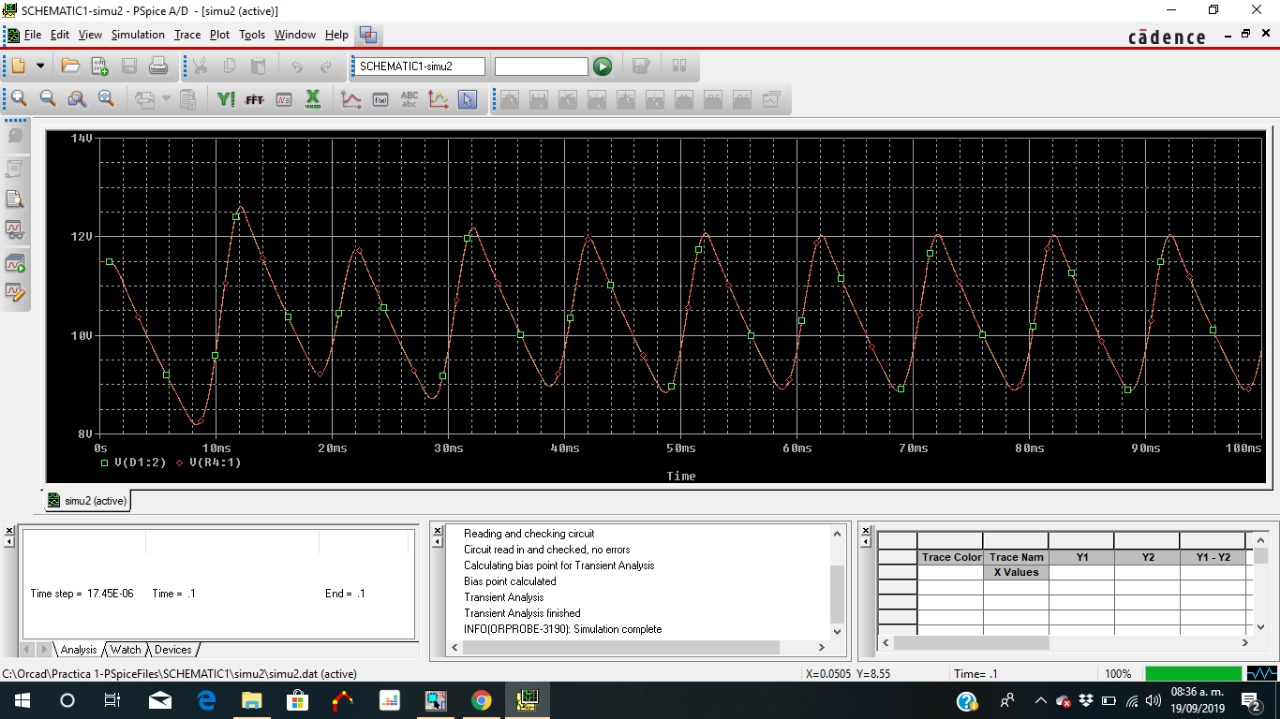
\includegraphics[scale=0.3]{6.jpeg}
\caption{Simulación: Tensión De Salida Del Rectificador}
\end{figure}

\newpage
\subsection{1.7.-Efecto De Las Inductancias De Red Sobre La Conmutación De Corriente}
En este punto se le añade un inductor de filtro en la etapa continua ya que las inductancias de la linea provocan que la continuación de corriente entre los diodos del rectificador no sea instantanea, para obtener el fenomedo de la conmutación de corriente entre diodos y analizar sus efectos sobre el funcionamiento del rectificador se utilizara en el circuito una fuente de 220v y 50 Hz, una bobina de 4mH, dos diodos (Dbreak), un inductor de 100A y la tierra, una vez armado el circuito se da a correr la simulación y en esta la tensión de salida forma la onda resultante seria casi nula durante la conducción del D2 y practicamente la de entrada sera durante la conducción del D1 y sin embargo la bobina no permite discontinuidades bruscas en la corriente que circula por ella de manera que mantiene simultaneamente a los dos diodos en conducción durante un tiempo nos despreciable y por ultimo durante todo ese tiempo la salida permanece cortocircuitada por el diodo D2, Produciendose la perdida de tensión que puede apreciarse en la siguiente imagén de la simulación el cual fue fomentada junto el circuito.
\begin{figure}[hbtp]
\centering
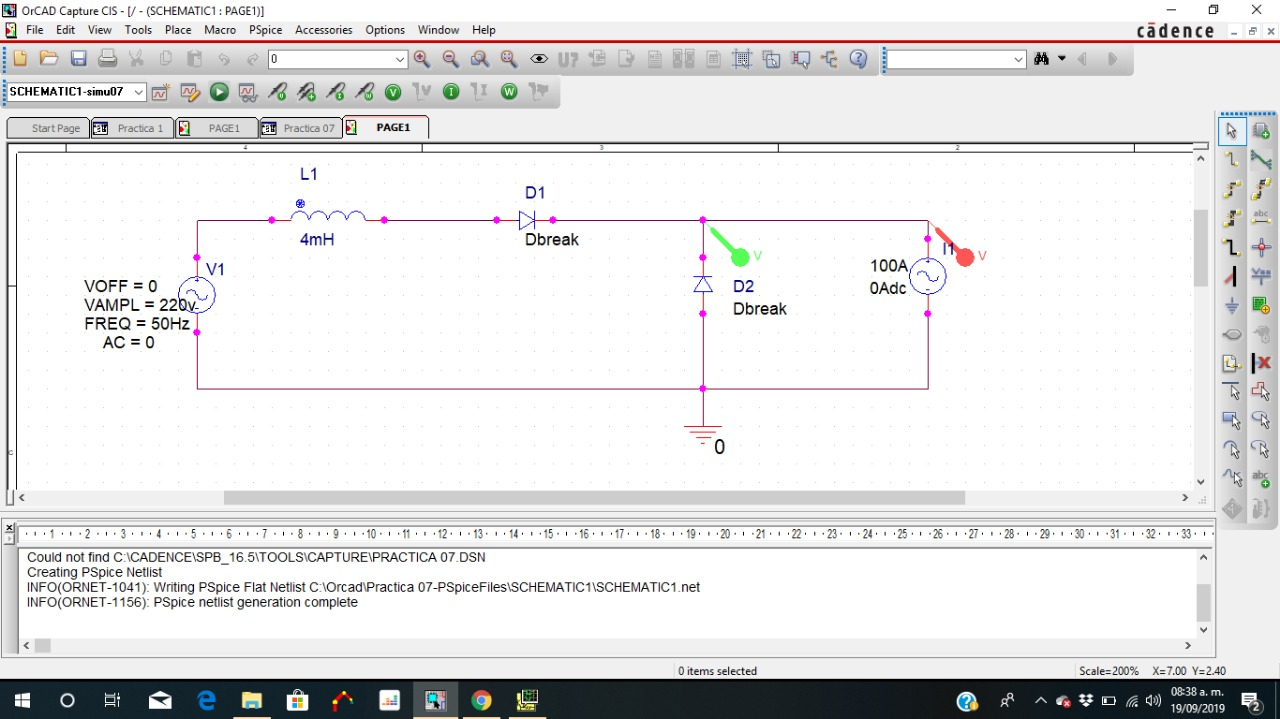
\includegraphics[scale=0.3]{07.jpeg}
\caption{Circuito Básico De Conmutación Entre Diodos}
\end{figure}
\begin{figure}[hbtp]
\centering
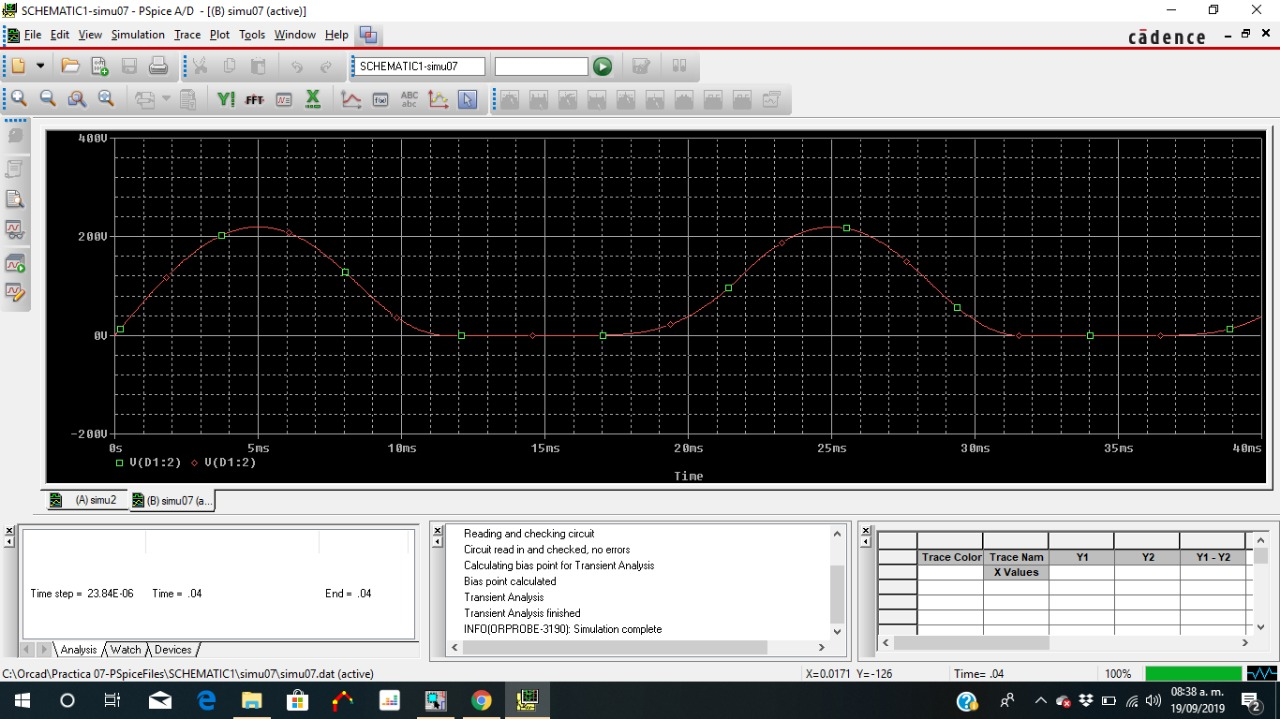
\includegraphics[scale=0.3]{7.jpeg}
\caption{Simulación: Tensión De Salida Cuando La Conmutación Entre Diodos Es Prácticamente Instantánea}
\end{figure}

\newpage
\section{Resultados}
los resultados de esta practica se lograron obtener como se esperaba mediante las simulaciones que se motraran a continuación:
\begin{figure}[hbtp]
\centering
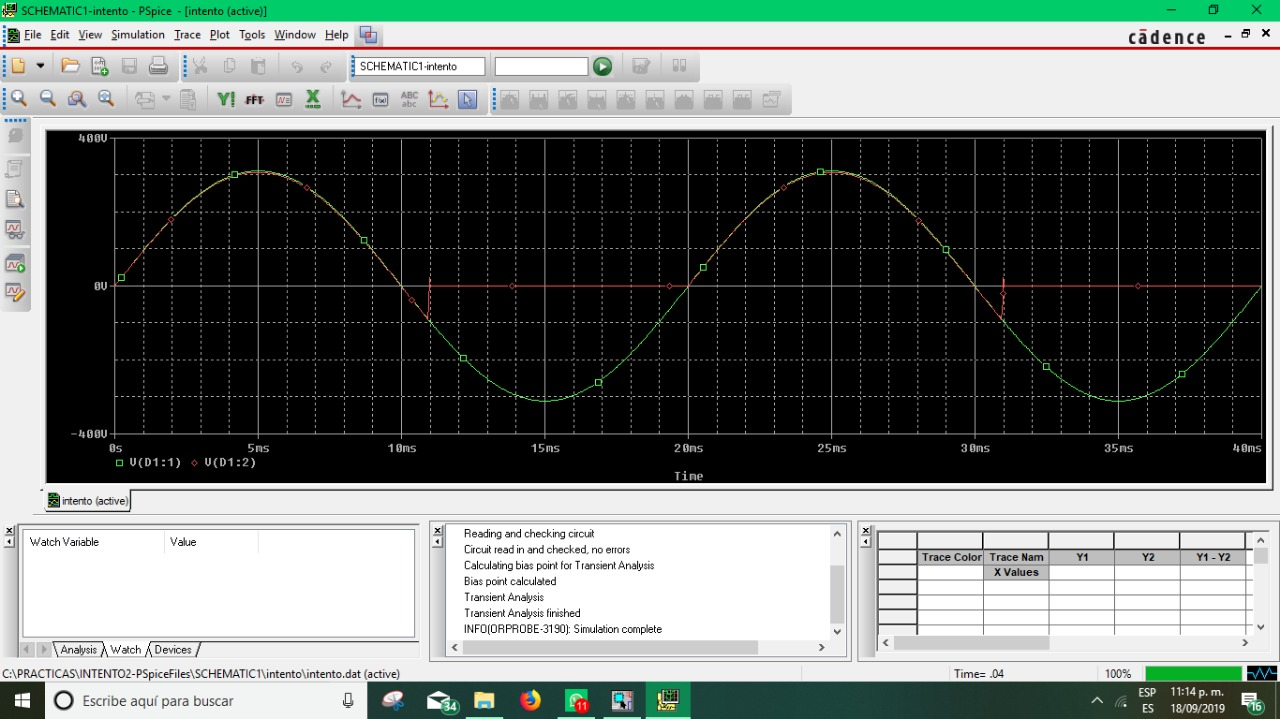
\includegraphics[scale=0.3]{2.jpeg}
\caption{ Simulación 1.2: Tensiones De Entrada Y De Salida Del Rectificador}
\end{figure}
\begin{figure}[hbtp]
\centering
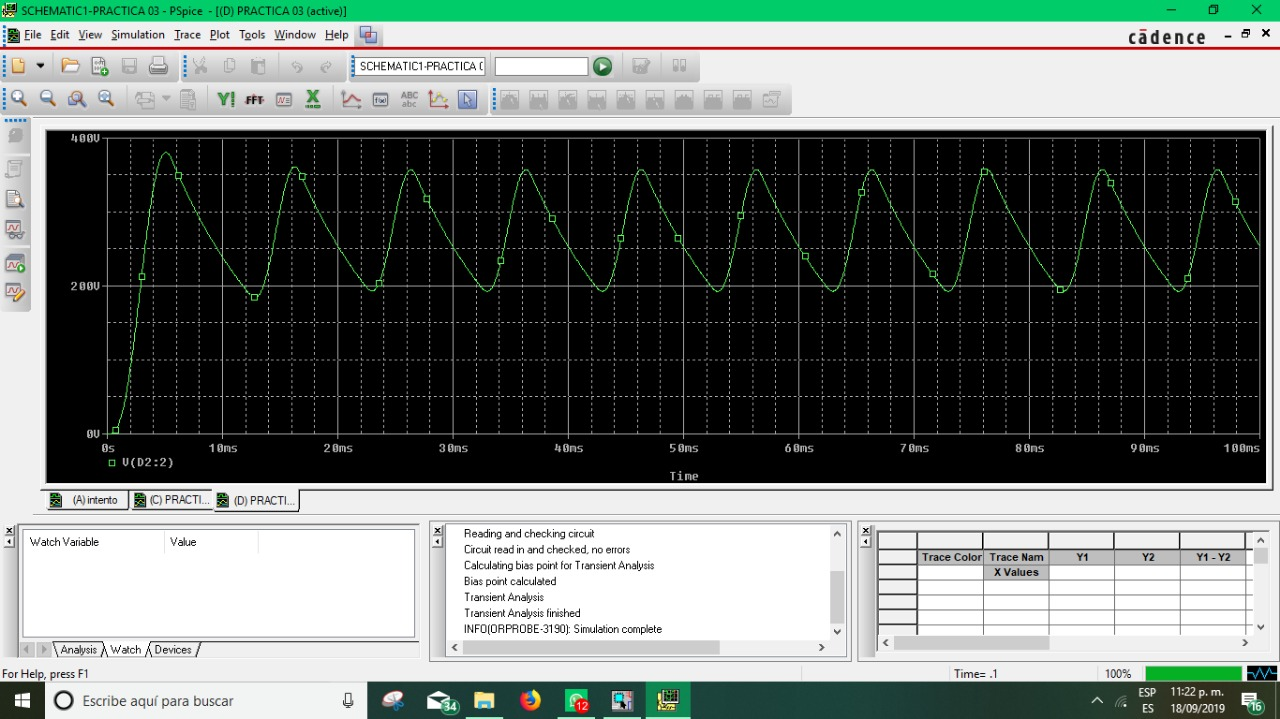
\includegraphics[scale=0.3]{3.jpeg}
\caption{Simulación 1.3: Tensión De Salida Del Rectificador}
\end{figure}
\begin{figure}[hbtp]
\centering
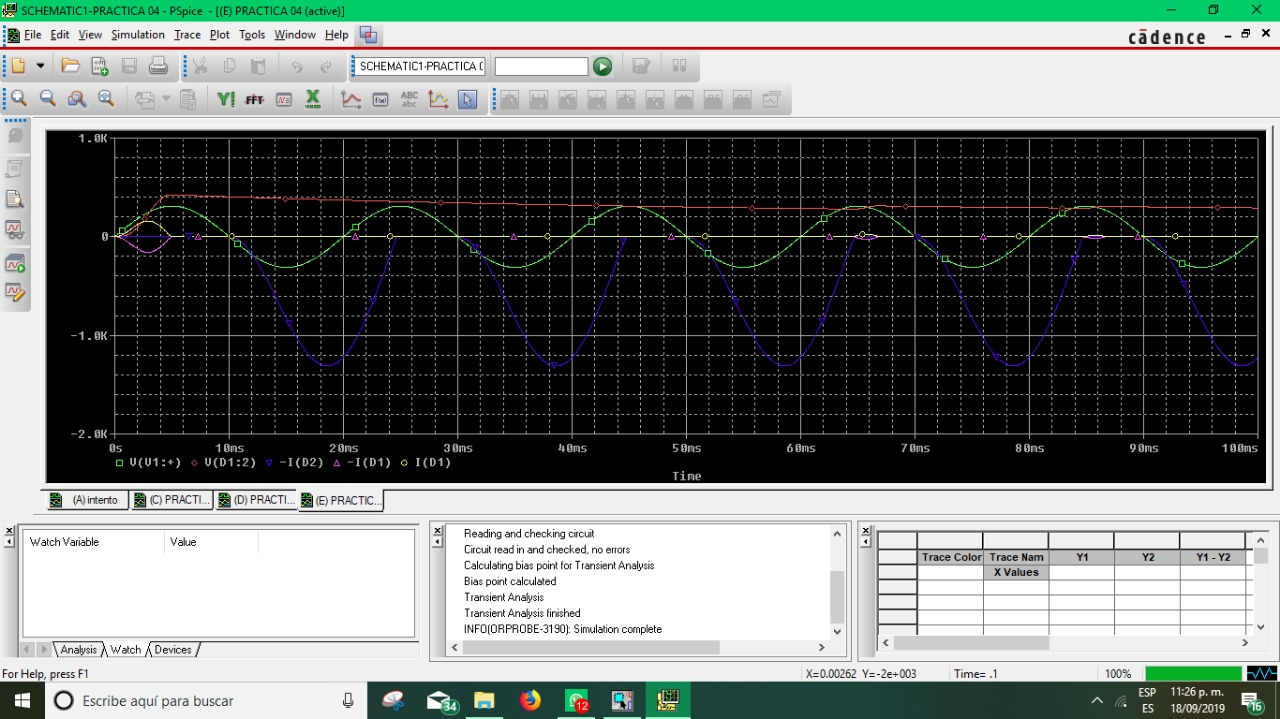
\includegraphics[scale=0.3]{4.jpeg}
\caption{Simulación 1.4: Rectificador De Tensión: Tensión De Salida Y En Los Condensadores}
\end{figure}
\begin{figure}[hbtp]
\centering
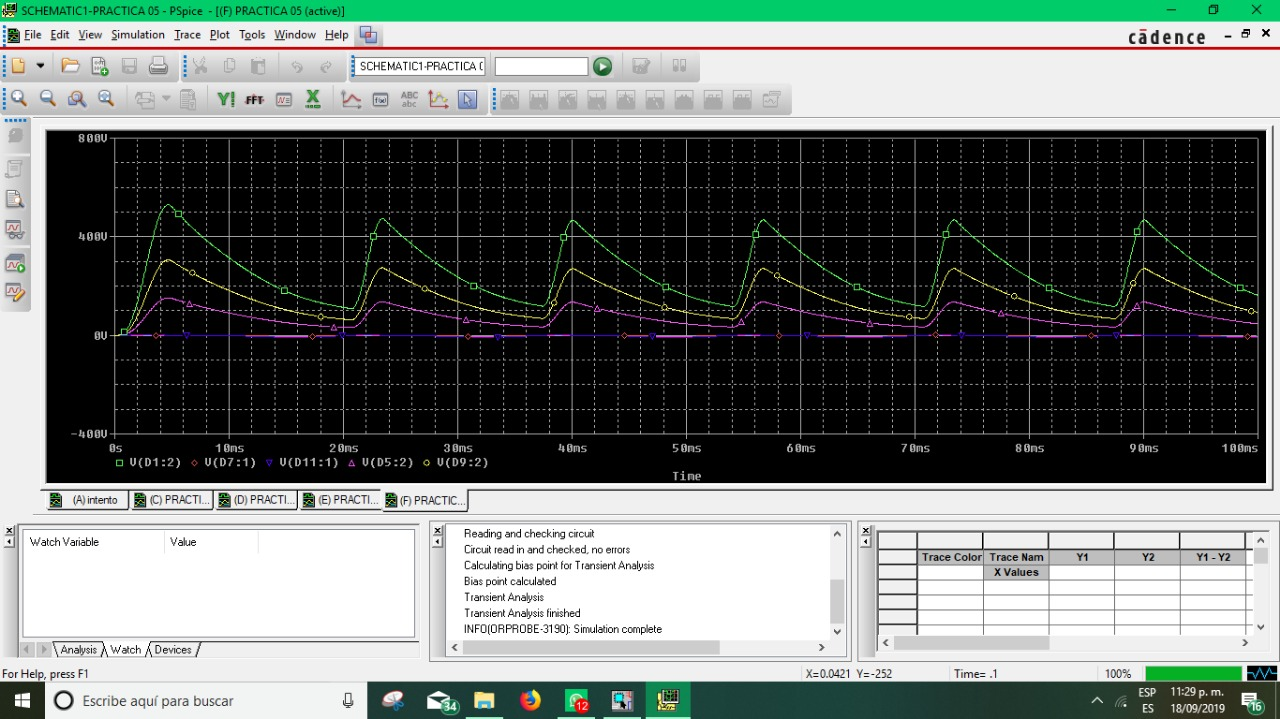
\includegraphics[scale=0.3]{5.jpeg}
\caption{Simulación 1.5: Corriente En Los Conductores De Línea Y Su Correspondiente Valor Eficaz}
\end{figure}
\begin{figure}[hbtp]
\centering
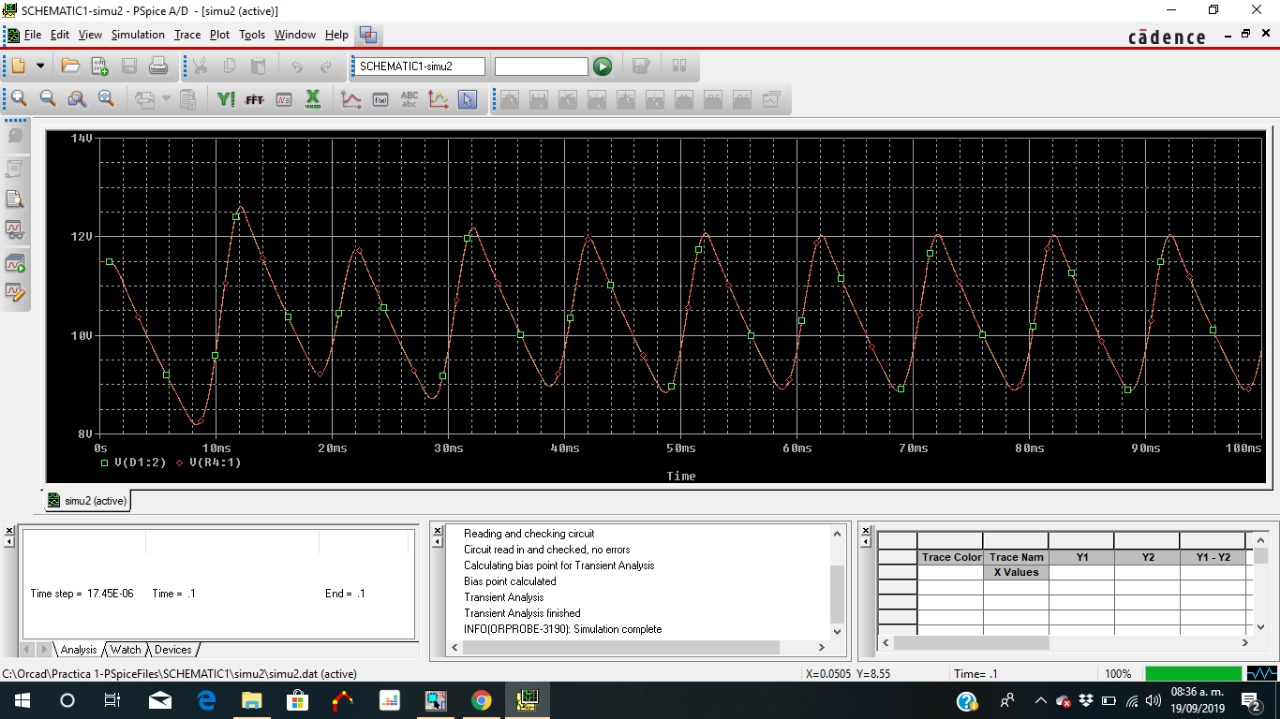
\includegraphics[scale=0.3]{6.jpeg}
\caption{Simulación 1.6: Tensión De Salida Del Rectificador}
\end{figure}
 \begin{figure}[hbtp]
\centering
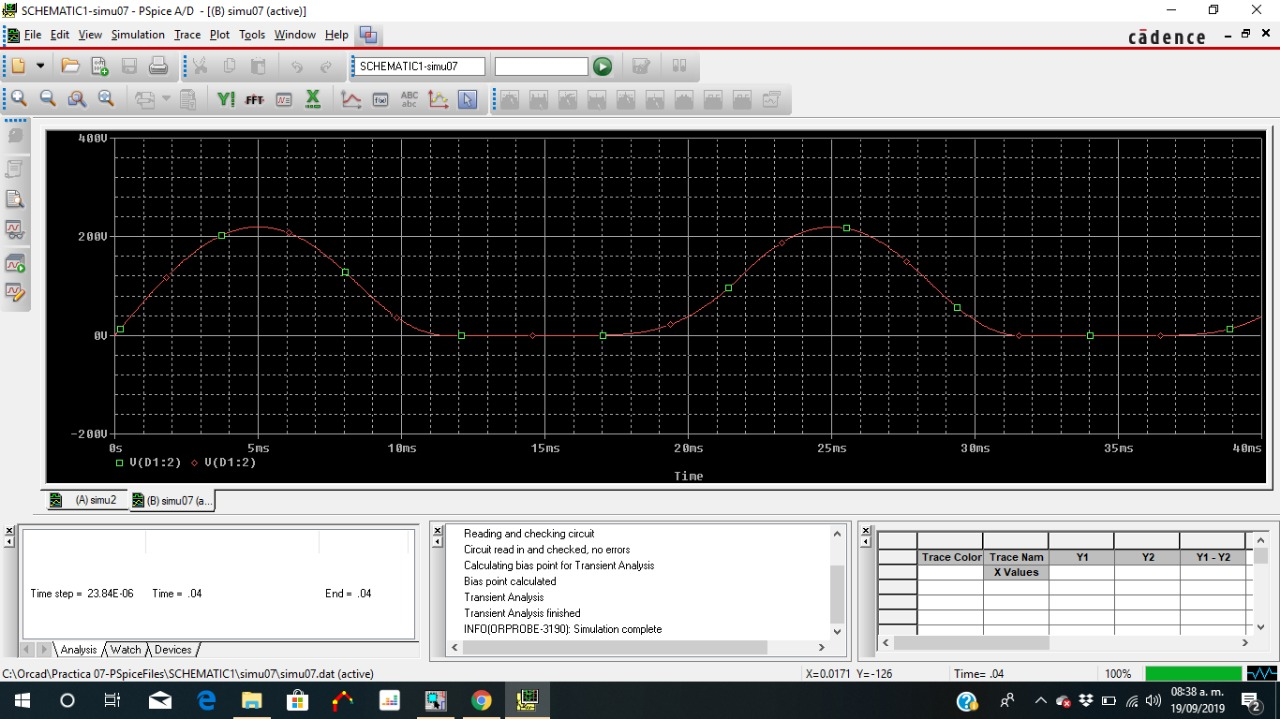
\includegraphics[scale=0.3]{7.jpeg}
\caption{Simulación 1.7: Tensión De Salida Cuando La Conmutación Entre Diodos Es Prácticamente Instantánea}
\end{figure}

\newpage
\section{Coclusiones}
En el desarrollo compredi como se comportan los multiples circuitos de rectificacion a su ves como el manejo  del programa "OrCad" en el ingreso de materiales, como solucionar los errores de nodos flotantes, los parametros de las simulaciones y cuando todo estaba perfectamente acomodado y corrias cada circuto el objetivo era comprender que funcion tenian estos mismos y compararlos con la información que venia en el archivo adjunto, fue una practica introductoria muy buena para una competencia de aprendizaje.
.

\pagebreak
\begin{LARGE}
Referencias\\\\
\end{LARGE}
\bibliography{Ev-1-1-Circuitos De Rectificacion No Controlados.bib}{https://www.uv.es/emaset/iep00/temas/IEP3-0607.pdf}
\bibliographystyle{plain}

\end{document}